\subsection{Linux Kernel: DRM}

\begin{frame}{DRM devices}
  \begin{itemize}
  \item UNIX-style devices are identified with major/minor numbers
    \begin{itemize}
    \item More details in the \code{makedev} manpage, using \code{dev_t} type
    \item Minor/major can be retrieved with \code{stat/fstat}
    \item DRM major in Linux is \textbf{226}
    \end{itemize}
  \item Two types of DRM devices exist:
    \begin{itemize}
    \item \textbf{Primary} nodes at \code{/dev/dri/card*} with minor \(< 128\)\\
    Used for display operations with the KMS (mode) interface
    \item \textbf{Render} nodes at \code{/dev/dri/renderD*} with minor \(\geq 128\)\\
    Used for render operations with a driver-specific interface
    \end{itemize}
  \item DRM devices can also be used by the kernel directly (internal clients):
    \begin{itemize}
    \item \textbf{fbdev} compatibility layer to provide \code{/dev/fb*} nodes
    \item Used by \textbf{fbcon} to provide virtual consoles
    \end{itemize}
  \item Userspace needs rights to open device nodes:
    \begin{itemize}
    \item Usually allowed via the \code{video} \textbf{group} or \textbf{Access Control Lists} (ACLs)
    \end{itemize}
  \end{itemize}
\end{frame}

\begin{frame}[fragile]{DRM driver identification and capabilities}
  \begin{itemize}
  \item Driver-specific \textbf{name and version} (major/minor/patchlevel) can be queried:%
  \begin{minted}[fontsize=\small]{console}
struct drm_version version = { ... };
ret = ioctl(drm_fd, DRM_IOCTL_VERSION, &version);
  \end{minted}
  \item Drivers expose specific \textbf{capabilities}, that can be queried:
  \begin{minted}[fontsize=\small]{console}
struct drm_get_cap get_cap = { 0 };
get_cap.capability = DRM_CAP_DUMB_BUFFER;
ret = ioctl(drm_fd, DRM_IOCTL_GET_CAP, &get_cap);
  \end{minted}
  \item The kernel \textbf{must} be informed of client support for some features:
  \begin{minted}[fontsize=\small]{console}
struct drm_set_client_cap client_cap = { 0 };
client_cap.capability = DRM_CLIENT_CAP_UNIVERSAL_PLANES;
client_cap.value = 1;
ret = ioctl(drm_fd, DRM_IOCTL_SET_CLIENT_CAP, &client_cap);
  \end{minted}
  \item Driver and client capabilities defined in Linux's \kfile{include/uapi/drm/drm.h}
  \end{itemize}
\end{frame}

\begin{frame}[fragile]{DRM master, magic and authentication}
  \begin{itemize}
  \item Multiple userspace clients can open the same primary device node
  \item Only the \textbf{master} client is allowed to configure display (KMS)
  \item Master is exclusive and can be \textbf{acquired} and \textbf{dropped} (VT switching):
  \begin{minted}[fontsize=\small]{console}
ret = ioctl(drm_fd, DRM_IOCTL_SET_MASTER, NULL);
ret = ioctl(drm_fd, DRM_IOCTL_DROP_MASTER, NULL);
  \end{minted}
  \item Requires \code{CAP_SYS_ADMIN} Linux capability, see \code{capabilities} man page\\
    \textit{usually reserved to the root super user}
  \item Some operations can be allowed on trusted clients with \textbf{magic authentication}:
    \begin{itemize}
      \item Mostly used before render nodes or for allocating buffers on another process
    \end{itemize}
  \begin{enumerate}
  \item Client \textit{foo} gets its client-specific magic:
  \begin{minted}[fontsize=\small]{console}
struct drm_auth auth = { 0 };
ret = ioctl(drm_fd, DRM_IOCTL_GET_MAGIC, &auth);
  \end{minted}
  \item Client \textit{foo} sends \code{auth.magic} to master client \textit{bar} (via IPC)
  \item Master client \textit{bar} authenticates client \textit{foo}:
  \begin{minted}[fontsize=\small]{console}
ret = ioctl(drm_fd, DRM_IOCTL_AUTH_MAGIC, &auth);
  \end{minted}
  \end{enumerate}
  \end{itemize}
\end{frame}

\begin{frame}[fragile]{DRM memory management}
  \begin{itemize}
  \item The \textbf{Graphics Execution Manager} (GEM) handles memory in DRM
  \item Used both by KMS and render drivers, with specific backends:
    \begin{itemize}
    \item \textbf{CMA}: Contiguous Memory Allocator (reserved area at boot)
    \item \textbf{Shmem}: Shared system memory (anonymous pages)
    \item \textbf{Vram}: Video RAM, using the \textbf{Translation Table Manager} (TTM)
    \end{itemize}
  \item Ensures buffers \textbf{coherency} on access (cache management)
  \item Allocated buffers are identified with a unique \textbf{handle} number
  \item In KMS, the \textbf{dumb buffer} API exposes memory operations:
    \begin{itemize}
    \item For memory used for \textbf{scanout framebuffers}
    \item Drivers calculate aligned pitch/stride and size based on dimensions and bpp
    \item Sometimes too limiting (e.g. multi-planar formats)
    \end{itemize}
  \item More details in the \textit{drm-memory} man page
  \item Drivers sometimes expose extra \code{ioctls} for more advanced needs
  \end{itemize}
\end{frame}

\begin{frame}[fragile]{DRM KMS dumb buffer API}
  \begin{itemize}
  \item \textbf{Allocating} from \code{width}, \code{height} and \code{bpp}, returning \code{handle}, \code{pitch} and \code{size}:\\
  \begin{minted}[fontsize=\small]{console}
struct drm_mode_create_dumb create_dumb = { ... };
ret = ioctl(drm_fd, DRM_IOCTL_MODE_CREATE_DUMB, &create_dumb);
  \end{minted}
  \item \textbf{Destroying} an allocated buffer:
  \begin{minted}[fontsize=\small]{console}
struct drm_mode_destroy_dumb destroy_dumb = { .handle = ..., };
ret = ioctl(drm_fd, DRM_IOCTL_MODE_DESTROY_DUMB, &destroy_dumb);
  \end{minted}
  \item \textbf{Preparing a mapping} in user memory for a buffer, returning an \code{offset}:
  \begin{minted}[fontsize=\small]{console}
struct drm_mode_map_dumb map_dumb = { .handle = ..., };
ret = ioctl(drm_fd, DRM_IOCTL_MODE_MAP_DUMB, &map_dumb);
  \end{minted}
  \item \textbf{Mapping memory} to userspace using the \code{offset}:
  \begin{minted}[fontsize=\small]{console}
map = mmap(NULL, create_dumb.size, PROT_READ | PROT_WRITE, MAP_SHARED,
           drm_fd, map_dumb.offset);
  \end{minted}
  \item \textbf{Unmapping} memory after use:
  \begin{minted}[fontsize=\small]{console}
munmap(map, create_dumb.size);
  \end{minted}
  \end{itemize}
\end{frame}

\begin{frame}[fragile]{DRM FourCCs and modifiers}
  \begin{itemize}
  \item DRM has its own representation of \textbf{pixel formats}, with FourCC codes (on 32 bits)
  \item Defined in the \kfile{include/uapi/drm/drm_fourcc.h} header
  \item They can specify up to 4 distinct \textbf{data planes} for color components
  \item Pixel formats are named "MSB-to-LSB" and specified in \textbf{little-endian} order\\
  \textit{LSB comes first in memory in little-endian}
  \item For instance, \code{DRM_FORMAT_XRGB8888} has the \code{B} byte first in memory\\
  \textit{Memory order is independent from the CPU or hardware endianness}
  \item A format \textbf{modifier} (on 64 bits) indicates the pixel order in memory
  \item \code{DRM_FORMAT_MOD_LINEAR} indicates raster order\\
  \textit{line-major left-to-right, top-to-bottom}
  \item Other modifiers are usually hardware-specific, often tiled\\
  (e.g. \code{DRM_FORMAT_MOD_VIVANTE_TILED})
  \end{itemize}
\end{frame}

\begin{frame}[fragile]{DRM KMS resources probing}
  \begin{itemize}
  \item KMS hardware resources are exposed through the following entities:
    \begin{itemize}
    \item Connectors
    \item Encoders
    \item CRTCs
    \item Planes: primary, overlay and cursor
    \item Framebuffers
    \end{itemize}
  \item Each resource instance is identified with a unique \textbf{identification number}
  \item The list of resource ids is retrieved with:
  \begin{minted}[fontsize=\small]{console}
struct drm_mode_card_res res = { ... };
ret = ioctl(drm_fd, DRM_IOCTL_MODE_GETRESOURCES, &res);
  \end{minted}
  \item Plane ids (that were introduced later) are retrieved with:
  \begin{minted}[fontsize=\small]{console}
struct drm_mode_get_plane_res res = { ... };
ret = ioctl(drm_fd, DRM_IOCTL_MODE_GETPLANERESOURCES, &res);
  \end{minted}
  \item Resource ids are used with subsequent resource-specific calls
  \end{itemize}
\end{frame}

\begin{frame}[fragile]{DRM KMS connector probing}
  \begin{itemize}
  \item The starting point to configure a KMS pipeline is the connector
  \item Current connector state is probed with:
  \begin{minted}[fontsize=\small]{console}
struct drm_mode_get_connector get_connector = { .connector_id = ... };
ret = ioctl(drm_fd, DRM_IOCTL_MODE_GETCONNECTOR, &get_connector);
  \end{minted}
  \item \code{struct drm_mode_get_connector} exposes various information:
    \begin{itemize}
    \item Connector type and connection state
    \item Possible encoders, currently-attached encoder
    \item Available modes and physical monitor size
    \end{itemize}
  \item Probing modes triggers EDID read: optional and usually quite slow
  \end{itemize}
\end{frame}

\begin{frame}[fragile]{DRM KMS modes}
  \begin{itemize}
  \item A display mode is represented as a \code{struct drm_mode_modeinfo} in DRM
  \item Members: \code{clock}, \code{[hv]display}, \code{[hv]sync_start}, \code{[hv]sync_end}, \code{[hv]total} and \code{flags} for signal-specific details (polarities)
  \item Diagram from \kfile{include/drm/drm_modes.h}:
  \begin{minted}[fontsize=\small]{console}
         Active                 Front           Sync           Back
         Region                 Porch                          Porch
<-----------------------><----------------><-------------><-------------->
  //////////////////////|
 ////////////////////// |
//////////////////////  |..................               ................
                                           _______________
<----- [hv]display ----->
<------------- [hv]sync_start ------------>
<--------------------- [hv]sync_end --------------------->
<-------------------------------- [hv]total ----------------------------->*
  \end{minted}
  \end{itemize}
\end{frame}

\begin{frame}[fragile]{DRM KMS encoder probing}
  \begin{itemize}
  \item The next step is to find which CRTC id can be used with the connector
  \item The encoder is the link between the connector and CRTC
  \item Current encoder state can be probed with:
  \begin{minted}[fontsize=\small]{console}
struct drm_mode_get_encoder get_encoder = { .encoder_id = ... };
ret = ioctl(drm_fd, DRM_IOCTL_MODE_GETENCODER, &get_encoder);
  \end{minted}
  \item \code{struct drm_mode_get_connector} exposes some information:
    \begin{itemize}
    \item Encoder type
    \item Possible CRTCs, currently-attached CRTC
    \end{itemize}
  \item This allows selecting the CRTC to use for the connector!
  \end{itemize}
\end{frame}

\begin{frame}[fragile]{DRM KMS framebuffer management}
  \begin{itemize}
  \item Framebuffers in DRM are described with a number of parameters:
    \begin{itemize}
    \item Picture-wide: \code{width}, \code{height}, \code{pixel_format}
    \item Plane-specific: GEM \code{handle}, \code{pitch}, \code{offset} and \code{modifier}
    \end{itemize}
  \item Up to 4 memory planes are supported (depending on the format)
  \item Allows supporting a wide range of possible configurations
  \item Flags are passed to indicate that modifiers or interlaced scan are used
  \item Framebuffers are registered from their parameters, returning a \code{fb_id}:
  \begin{minted}[fontsize=\small]{console}
struct drm_mode_fb_cmd2 fb_cmd2 = { ... };
ret = ioctl(drm_fd, DRM_IOCTL_MODE_ADDFB2, &fb_cmd2);
  \end{minted}
  \item They are destroyed using the \code{fb_id}:
  \begin{minted}[fontsize=\small]{console}
unsigned int fb_id = fb_cmd2.fb_id;
ret = ioctl(drm_fd, DRM_IOCTL_MODE_RMFB, &fb_id);
  \end{minted}
  \end{itemize}
\end{frame}

\begin{frame}[fragile]{DRM KMS CRTC configuration (legacy)}
  \begin{itemize}
  \item The pipeline can then be configured with the connector and the CRTC
  \item The current CRTC configuration can be retrieved with:
  \begin{minted}[fontsize=\small]{console}
struct drm_mode_crtc crtc = { .crtc_id = ... };
ret = ioctl(drm_fd, DRM_IOCTL_MODE_GETCRTC, &crtc);
  \end{minted}
  \item The CRTC is configured with the connector id
  \begin{minted}[fontsize=\small]{console}
struct drm_mode_crtc crtc = { .crtc_id = ... };
ret = ioctl(drm_fd, DRM_IOCTL_MODE_SETCRTC, &crtc);
  \end{minted}
  \item A mode and a framebuffer can be set (previous setup used otherwise)\\
  \textit{mandatory if the CRTC was unused before}
  \item The kernel will automatically select the best encoder for the connector and CRTC
  \item \textbf{Legacy and deprecated} way to do modesetting: only concerns the primary plane
  \end{itemize}
\end{frame}

\begin{frame}[fragile]{DRM KMS page flipping (legacy)}
  \begin{itemize}
  \item Page flipping is the action of switching the CRTC to another framebuffer\\
  \textit{only concerns the primary plane}
  \item An event can be requested when the flip happens
  \item Can be scheduled at different times (specified with \code{flags}):
    \begin{itemize}
    \item At a specified vblank target (absolute or relative) to avoid tearing
    \item As soon as possible (asynchronously) if supported
    \end{itemize}
  \begin{minted}[fontsize=\small]{console}
struct drm_mode_crtc_page_flip page_flip = { .crtc_id = ..., .fb_id = ... };
ret = ioctl(drm_fd, DRM_IOCTL_MODE_PAGE_FLIP, &page_flip);
  \end{minted}
  \item \textbf{Legacy and deprecated}: limited to the primary plane
  \end{itemize}
\end{frame}

\begin{frame}[fragile]{DRM KMS overlay plane configuration (legacy)}
  \begin{itemize}
  \item Overlay planes are configured separately from the CRTC main plane
  \item The current state of a plane can be retrieved with:
  \begin{minted}[fontsize=\small]{console}
struct drm_mode_get_plane get_plane = { .plane_id = ... };
ret = ioctl(drm_fd, DRM_IOCTL_MODE_GETPLANE, &get_plane);
  \end{minted}
  \item Provides possible CRTCs, current framebuffer and supported formats
  \item Planes are configured with source and destination parameters:
    \begin{itemize}
    \item \code{crtc_[xywh]}: On-CRTC position and dimensions
    \item \code{src_[xywh]}: In-framebuffer position and dimensions (source clipping area)
    \end{itemize}
  \item Configuration takes place with:
  \begin{minted}[fontsize=\small]{console}
struct drm_mode_set_plane set_plane = { .plane_id = ... };
ret = ioctl(drm_fd, DRM_IOCTL_MODE_SETPLANE, &set_plane);
  \end{minted}
  \item \textbf{Legacy and deprecated}: not synchronized to vblank or page flip
  \end{itemize}
\end{frame}

\begin{frame}[fragile]{DRM KMS cursor configuration and position (legacy)}
  \begin{itemize}
  \item Cursor planes have a separate dedicated legacy API
  \item Configured per-CRTC with a GEM \code{handle} and dimensions (\code{width}, \code{height})\\
  \textit{a zero GEM \code{handle} deconfigures and removes the cursor}
  \item Only supports the \code{DRM_FORMAT_ARGB8888} format (not configurable)
  \item Using a single \code{ioctl} with the \code{flags} field for the operation
  \begin{minted}[fontsize=\small]{console}
struct drm_mode_cursor cursor = { .flags = DRM_MODE_CURSOR_BO,
                                  .crtc_id = ...};
ret = ioctl(drm_fd, DRM_IOCTL_MODE_CURSOR, &cursor);
  \end{minted}
  \item Once configured, the cursor can be moved to \code{x}, \code{y} on-CRTC coordinates
  \begin{minted}[fontsize=\small]{console}
struct drm_mode_cursor cursor = { .flags = DRM_MODE_CURSOR_MOVE,
                                  .crtc_id = ... };
ret = ioctl(drm_fd, DRM_IOCTL_MODE_CURSOR, &cursor);
  \end{minted}
  \item \code{DRM_IOCTL_MODE_CURSOR2} variant provides cursor hotspot for virtual machines
  \end{itemize}
\end{frame}

\begin{frame}[fragile]{DRM event notification and wait}
  \begin{itemize}
  \item DRM provides an event notification mechanism for \textbf{vblank} and \textbf{page flip done}
  \item Available through the primary (KMS) file descriptor
  \item Can be used with \code{poll} and \code{select} (integrated in main loop)
  \item Events with a \code{struct drm_event} base are read using \code{read}
  \item Expand to \code{struct drm_event_vblank} for vblank and page flip done events\\
    \textit{only complete events are returned, so the buffer must be large enough}
  \item Events can be requested at page flip time or explicitly:
  \begin{minted}[fontsize=\small]{console}
union drm_wait_vblank wait_vblank = { .request = ... };
ret = ioctl(drm_fd, DRM_IOCTL_WAIT_VBLANK, &wait_vblank);
  \end{minted}
  \item A blocking wait for an absolute or relative vblank sequence can also be requested\\
  \textit{using the same \code{ioctl} and dedicated \code{request.type} values}
  \end{itemize}
\end{frame}

\begin{frame}[fragile]{DRM KMS object properties}
  \begin{itemize}
  \item KMS objects expose generic (or driver-specific) properties with names and values
  \textit{concerns \textbf{connectors}, \textbf{CRTCs} and \textbf{planes}}
    \begin{itemize}
    \item \textbf{Range} properties: limits for the value (signed or unsigned)
    \item \textbf{Enum} properties: fixed values with associated names for the values
    \item \textbf{Blob} properties: raw data with a given length
    \end{itemize}
  \item Properties have a \textbf{unique identifier across objects}, details can be queried:
  \begin{minted}[fontsize=\small]{console}
struct drm_mode_obj_get_property get_property = { .prop_id = ... }
ret = ioctl(drm_fd, DRM_IOCTL_MODE_GETPROPERTY, &get_property);
  \end{minted}
  \item Registered properties of an object can be retrieved using:
  \begin{minted}[fontsize=\small]{console}
struct drm_mode_obj_get_properties get_properties = { .obj_id = ... }
ret = ioctl(drm_fd, DRM_IOCTL_MODE_OBJ_GETPROPERTIES, &get_properties);
  \end{minted}
  \item The \code{value} of a property can be assigned with:
  \begin{minted}[fontsize=\small]{console}
struct drm_mode_obj_set_property set_property = { .obj_id = ..., .prop_id = ... }
ret = ioctl(drm_fd, DRM_IOCTL_MODE_OBJ_SETPROPERTY, &set_property);
  \end{minted}
  \item Blob properties need to be created and destroyed (with their own identifier)
  \end{itemize}
\end{frame}

\begin{frame}[fragile]{DRM KMS atomic}
  \begin{itemize}
  \item The legacy API comes with major design issues:
    \begin{itemize}
    \item Overlay and cursor plane updates are applied instantly (tearing)
    \item Plane updates cannot be synchronized together (intermediate states)
    \item No way to check that setup is valid before applying it
    \end{itemize}
  \item The atomic API lifts these restrictions with a new paradigm:
    \begin{itemize}
    \item Objects are configured based on their KMS properties\\
    \textit{values are affected to each changed property}
    \item Property changes of different objects are grouped in an \textbf{atomic commit}
    \item Planes are handled regardless of their type (primary, overlay, cursor)
    \item Commits can be marked for test only: checked but not applied
    \item Changes are applied at next vblank, unless marked asynchronous
    \end{itemize}
  \begin{minted}[fontsize=\small]{console}
struct drm_mode_atomic atomic = { ... }
ret = ioctl(drm_fd, DRM_IOCTL_MODE_ATOMIC, &atomic);
  \end{minted}
  \item Unless marked non-blocking, the \code{ioctl} returns when changes are applied
  \item A page flip event can also be requested
  \end{itemize}
\end{frame}

\begin{frame}[fragile]{DRM KMS atomic common properties}
  \begin{itemize}
  \item Common properties used to configure \textbf{connectors}:
    \begin{itemize}
    \item \code{CRTC_ID}: id of the CRTC to bind with the connector
    \end{itemize}
  \item Common properties used to configure \textbf{CRTCs}:
    \begin{itemize}
    \item \code{ACTIVE}: whether the CRTC is in use
    \item \code{MODE_ID}: id of the property blob with the \code{struct drm_mode_modeinfo} mode
    \end{itemize}
  \item Common properties used to configure \textbf{planes}:
    \begin{itemize}
    \item \code{FB_ID}: id of the framebuffer to bind with the plane
    \item \code{CRTC_ID}: id of the CRTC to bind with the plane
    \item \code{CRTC_[XYWH]}: on-CRTC position and dimensions of the plane
    \item \code{SRC_[XYWH]}: in-framebuffer position and dimensions (source clipping area)
    \end{itemize}
  \item Common properties used to probe \textbf{planes}:
    \begin{itemize}
    \item \code{TYPE}: type of the plane (primary/overlay/cursor)
    \item \code{IN_FORMATS}: list of supported formats/modifiers
    \end{itemize}
  \end{itemize}
\end{frame}

\begin{frame}[fragile]{DRM KMS atomic driver walkthrough}
  \begin{itemize}
  \item A state-of-the-art DRM KMS driver: \code{vc4} at \kdir{drivers/gpu/drm/vc4}\\
  \textit{integrates both DRM KMS and render}
  \item Entry point at \kfile{drivers/gpu/drm/vc4/vc4_drv.c}
  \item Dedicated documentation: \url{https://dri.freedesktop.org/docs/drm/gpu/vc4.html}
  \end{itemize}
\end{frame}

\begin{frame}[fragile]{DRM render generalities}
  \begin{itemize}
  \item DRM render drivers have their own \textbf{driver-specific API}\\
    \textit{unlike KMS, render hardware abstraction is done in userspace}
  \item Their API is exposed through custom \code{ioctls}
  \item Can be associated with a KMS driver (e.g. \code{vc4}) or separate (e.g. \code{v3d})
  \item Drivers handle memory, job submission and scheduling, interrupts
  \item DRM has a common scheduler (from AMD) in \kdir{drivers/gpu/drm/scheduler}
  \item Usual operations:
    \begin{itemize}
    \item Managing buffer objects (BOs) of different types (create, destroy, mmap)\\
    \textit{using GEM under the hood}
    \item Submitting job data structures for programming the GPU (command lists)\\
    \textit{with a validation step to ensure its validity}
    \item Waiting for operations to complete
    \item Exposing performance-related information
    \end{itemize}
  \end{itemize}
\end{frame}

\begin{frame}[fragile]{DRM render driver walkthrough}
  \begin{itemize}
  \item A state-of-the-art DRM render driver: \code{v3d} at \kdir{drivers/gpu/drm/v3d}
  \item Entry point at \kfile{drivers/gpu/drm/v3d/v3d_drv.c}
  \item Dedicated documentation: \url{https://dri.freedesktop.org/docs/drm/gpu/v3d.html}
  \end{itemize}
\end{frame}

\begin{frame}[fragile]{DRM Prime zero-copy memory sharing (dma-buf)}
  \begin{itemize}
  \item Memory buffers often need to be shared between different devices\\
    \textit{e.g. DRM KMS and DRM render but also concerns V4L2 for media devices}
  \item The kernel-wide \code{dma-buf} API allows exporting and importing buffers
  \item Buffers are represented as \textbf{file descriptors} in userspace\\
    \textit{file descriptors can be shared between programs via IPC}
  \item DRM exposes dma-buf via the \textbf{DRM Prime} API
  \item DRM prime exports a GEM \code{handle} to a returned \code{fd}:
  \begin{minted}[fontsize=\small]{console}
struct drm_prime_handle prime_handle = { .handle = ... }
ret = ioctl(drm_fd, DRM_IOCTL_PRIME_HANDLE_TO_FD, &prime_handle);
  \end{minted}
  \item And vice-versa:
  \begin{minted}[fontsize=\small]{console}
struct drm_prime_handle prime_handle = { .fd = ... }
ret = ioctl(drm_fd, DRM_IOCTL_PRIME_FD_TO_HANDLE, &prime_handle);
  \end{minted}
  \end{itemize}
\end{frame}

\begin{frame}[fragile]{DRM sync object fencing}
  \begin{itemize}
  \item In a multi-device pipeline with zero-copy, only scheduling is left to userspace\\
  \textit{each device signals completion and userspace moves on to the next}
  \item Fences were introduced to avoid the extra roundtrip in userspace:
    \begin{itemize}
    \item The flow of buffers between devices is usually known in advance
    \item The kernel can coordinate internally and trigger the next device
    \item Requires submitting all commands in advance with fences attached
    \end{itemize}
  \item DRM exposes fences via the \textbf{Sync object} API
  \item Sync objects contain one fence, exposed as a file descriptor
  \item The KMS atomic API and some render driver APIs take input fence fds
  \end{itemize}
\end{frame}

\begin{frame}[fragile]{DRM sync object fencing}
  \begin{itemize}
  \item Sync objects are created and destroyed with a \code{handle}:
  \begin{minted}[fontsize=\small]{console}
struct drm_syncobj_create syncobj_create = { 0 }
ret = ioctl(drm_fd, DRM_IOCTL_SYNCOBJ_CREATE, &syncobj_create);
  \end{minted}
  \begin{minted}[fontsize=\small]{console}
struct drm_syncobj_destroy syncobj_destroy = { .handle = syncobj_create.handle }
ret = ioctl(drm_fd, DRM_IOCTL_SYNCOBJ_DESTROY, &syncobj_destroy);
  \end{minted}
  \item An output fence's \code{fd} is exported from a device's sync object with:
  \begin{minted}[fontsize=\small]{console}
struct drm_syncobj_handle syncobj_handle = { .handle = handle, ... }
ret = ioctl(drm_fd, DRM_IOCTL_SYNCOBJ_HANDLE_TO_FD, &syncobj_handle);
  \end{minted}
  \item An input fence's \code{fd} is imported to a device's sync object with:
  \begin{minted}[fontsize=\small]{console}
struct drm_syncobj_handle syncobj_handle = { .handle = handle, .fd = fd }
ret = ioctl(drm_fd, DRM_IOCTL_SYNCOBJ_FD_TO_HANDLE, &syncobj_handle);
  \end{minted}
  \item Quite a recent feature, not yet available in V4L2 (media)
  \end{itemize}
\end{frame}

\begin{frame}[fragile]{DRM debug and documentation}
  \begin{itemize}
  \item \textbf{Debug message} using the \code{drm.debug} kernel cmdline argument:
    \begin{itemize}
    \item Detailed in the \kfile{include/drm/drm_print.h} header
    \item \code{drm.debug=0x17} for core, KMS, driver and atomic debug messages
    \end{itemize}
  \item Current \textbf{state debug} in debugfs: \code{cat /sys/kernel/debug/dri/0/state}
  \item Drivers expose \textbf{specific debugfs entries}
  \item \textbf{Debug utility}: \code{modetest} from \code{libdrm}
  \item \textbf{Community} contact:
    \begin{itemize}
    \item Mailing list: \code{dri-devel@lists.freedesktop.org}
    \item IRC channel: \code{#dri-devel} on the OFTC network
    \end{itemize}
  \item \textbf{Documentation} resources:
    \begin{itemize}
    \item Linux GPU Driver Developer’s Guide: \url{https://www.kernel.org/doc/html/latest/gpu/index.html}
    \item Man pages about userspace aspects: \code{drm}, \code{drm-kms}, \code{drm-memory}
    \end{itemize}
  \end{itemize}
\end{frame}

\begin{frame}{libdrm wrapper}
  \begin{itemize}
  \item Userspace access to DRM devices is wrapped with \textbf{libdrm}
  \item Exposes convenience wrappers, helpers and some data structures around \code{ioctls}
    \begin{itemize}
    \item For KMS support in the \code{libdrm.so} library
    \item For hardware-specific render drivers in dedicated libraries (e.g. \code{libdrm_nouveau.so})
    \end{itemize}
  \item Used by almost every userspace project dealing with DRM:\\
    \textit{weston, mutter, Xorg, mesa, etc}
  \end{itemize}

  \begin{center}
  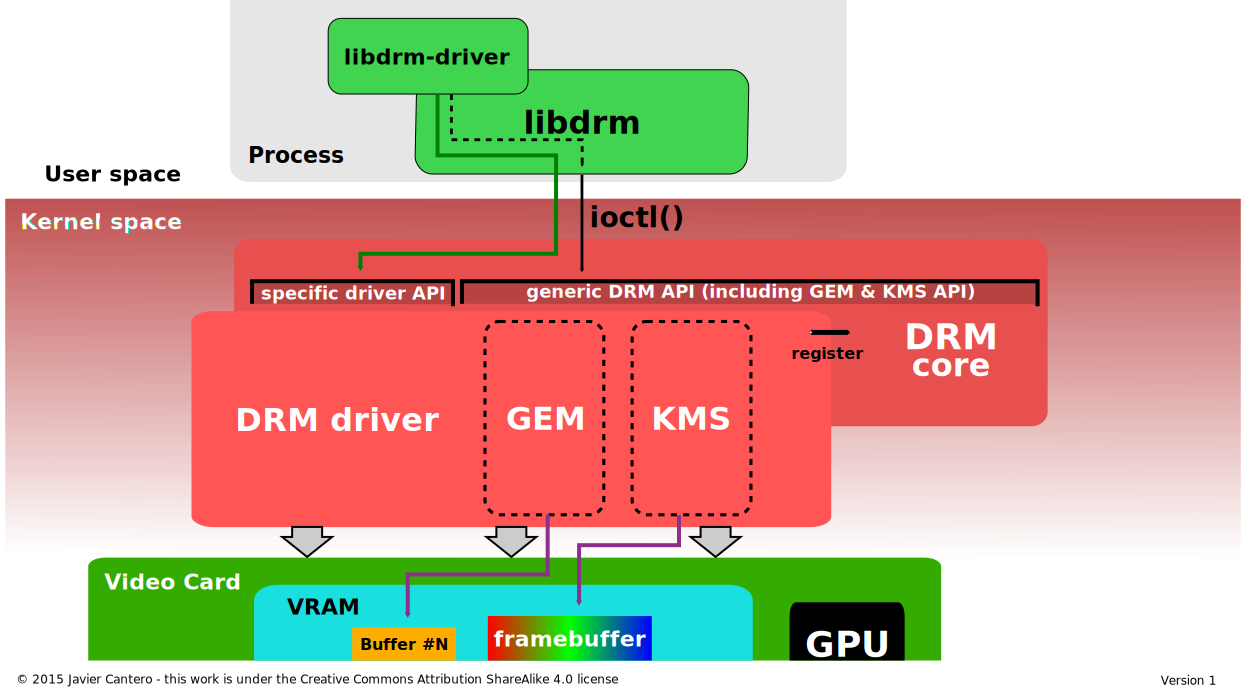
\includegraphics[width=0.5\textwidth]{slides/graphics-software-linux-drm/libdrm-userspace.pdf}
  \end{center}
\end{frame}
